\documentclass[twocolumn]{article}
\usepackage{cite}
\usepackage{hyperref}
\usepackage{graphicx}
\usepackage{tabularx}
\usepackage{booktabs}

\title{\textbf{Mapping the Intellectual Structure of Social Network Research: A Bibliometric Analysis of Three Journals}}
\author{\textbf{Pengjia Cui}}
\date{}

\begin{document}
	
	\maketitle
	
	\begin{abstract}
		This study presents a comprehensive bibliometric analysis of research published in three leading journals in the field of social network studies: \textit{Social Networks}, \textit{Journal of Complex Networks}, and \textit{Network Science}. Using data retrieved from the \textit{Web of Science} (WoS), we employ performance analysis, science mapping, and network analysis to examine the intellectual structure, research trends, and collaboration patterns within the domain. Our findings reveal key thematic clusters, influential publications, and evolving research trajectories. Additionally, we assess the impact of prolific authors and institutions while mapping co-authorship networks to understand patterns of scholarly collaboration. By integrating multiple bibliometric techniques, this study provides a structured overview of the field’s development, offering insights into emerging research areas and future directions in social and complex network studies.
	\end{abstract}
	
	\section{Introduction}\label{Introduction}
	
	Bibliometric analysis provides a systematic approach to understanding the intellectual landscape and research dynamics within a scientific field. By examining publication and citation patterns, scholars can gain insights into key research themes, methodological trends, and the evolution of scholarly discourse. In this study, we conduct a bibliometric analysis of three leading journals in social and complex network research—\textit{Social Networks}, \textit{Journal of Complex Networks}, and \textit{Network Science}—to map the intellectual structure of the field, identify key themes and trends, assess research impact, and analyze collaboration patterns.
	
	Specifically, this study aims to: (1) map the intellectual structure of social network research by examining citation networks and scholarly influences, (2) identify key themes and trends by analyzing keyword co-occurrence and thematic clusters across the three journals, (3) assess research impact by evaluating citation counts, influential publications, and contributions from prolific authors and institutions, and (4) analyze collaboration patterns by exploring co-authorship networks and institutional affiliations.
	
	To achieve these objectives, our analysis is structured into three main components. First, we conduct a performance analysis to assess publication trends, citation impact, and the contributions of leading scholars and institutions. Second, we implement science mapping techniques—including co-citation analysis, bibliographic coupling, and keyword co-occurrence analysis—to explore the thematic evolution and intellectual structure of the field. Finally, we perform a network analysis to examine collaboration patterns among researchers, institutions, and countries, uncovering structural properties of co-authorship and citation networks.
	
	By integrating these approaches, this study offers a structured overview of the current research landscape in social and complex network studies. While not exhaustive, it provides valuable insights into the development and diffusion of knowledge in the field, highlighting emerging research trajectories and potential future directions.
	
	Having defined the aims and scope of this study, the next step is to determine the bibliometric techniques that will allow us to systematically analyze the research landscape within \textit{Social Networks}, \textit{Journal of Complex Networks}, and Network Science. Following \cite{donthu_how_2021}, we categorize our approach into three primary analytical components: performance analysis, science mapping, and network analysis. Each technique is selected to directly align with our research objectives.
	
	\section{Bibliometric Techniques}\label{Bibliometric Techniques}
	
	To systematically analyze the intellectual structure of social network research, this study employs three interconnected bibliometric approaches: performance analysis, science mapping, and network analysis. Each method offers distinct yet complementary insights into the research landscape of the three selected journals.
	
	\textbf{Performance analysis} provides a quantitative assessment of research productivity and impact by examining publication trends, citation metrics, and the contributions of influential authors, institutions, and countries.
	
	\textbf{Science mapping} uncovers the thematic and conceptual structure of the field by identifying research clusters, keyword co-occurrence patterns, and intellectual influences through co-citation and bibliographic coupling analyses.
	
	\textbf{Network analysis} explores patterns of collaboration among authors, institutions, and countries, shedding light on the social and structural dynamics of knowledge production in social network research.
	
	By systematically integrating these three analytical components, this study provides a comprehensive and structured overview of social network research across the selected journals. The results will:
	
	\begin{itemize}
		\item Reveal historical and emerging research trends, highlighting shifts in dominant themes and methodological approaches.
		\item Identify key contributors and influential works, offering insights into the most impactful papers, prolific scholars, and leading institutions.
		\item Map collaborative networks, examining how scholars, institutions, and countries interact and contribute to the field.
	\end{itemize}
	
	Our multi-faceted approach ensures that the study not only quantifies research impact but also contextualizes the development of ideas, theories, and methodologies in social network research. The following sections describe each bibliometric technique in detail, outlining its purpose, methodology, data requirements, and analytical tools.
	
	\section{Performance Analysis}\label{Performance Analysis}
	
	Performance analysis in bibliometrics provides an overview of research productivity, citation impact, and contributions of authors, institutions, and countries. It helps quantify the most influential publications, prolific researchers, and overall research trends in \textit{Social Networks}, \textit{Journal of Complex Networks}, and \textit{Network Science}.
	
	\subsection{Data Collection and Preprocessing}
	
	To ensure a comprehensive and accurate dataset for bibliometric analysis, we retrieved publication records from the Web of Science (WoS), limiting our selection to articles published in \textit{Social Networks}, \textit{Journal of Complex Networks}, and \textit{Network Science}. The search was structured to include only records explicitly affiliated with these journals, avoiding misclassification from unrelated sources. The full query links used for data extraction are provided below:
	
	\begin{itemize}
		\item \url{https://www.webofscience.com/wos/woscc/summary/8b9cb9e7-5920-4a8c-8957-1f45746eb38f-01449729f7/relevance/1}
		\item \url{https://www.webofscience.com/wos/woscc/summary/b70d5df8-5cd9-4064-8329-390221e5fcc0-014497387b/relevance/1}
		\item \url{https://www.webofscience.com/wos/woscc/summary/cfb2985d-4457-4214-85c1-4ee6224ffecb-014497425b/relevance/1}
	\end{itemize}
	
	Following data retrieval, a preprocessing step was conducted to refine the dataset. We verified that each record belonged to one of the three journals and removed any erroneous entries. Records with missing or incomplete metadata—such as missing publication years, authorship details, or incorrectly formatted citations—were excluded. These measures ensured that our analysis accurately reflected the scholarly output in these journals without distortions from irrelevant or unreliable data.
	
	\subsection{Publication Trends in Social Network Research}
	
	\begin{figure}[htbp]
		\centering
		\caption{Publication Trends}\label{fig.fig1}
		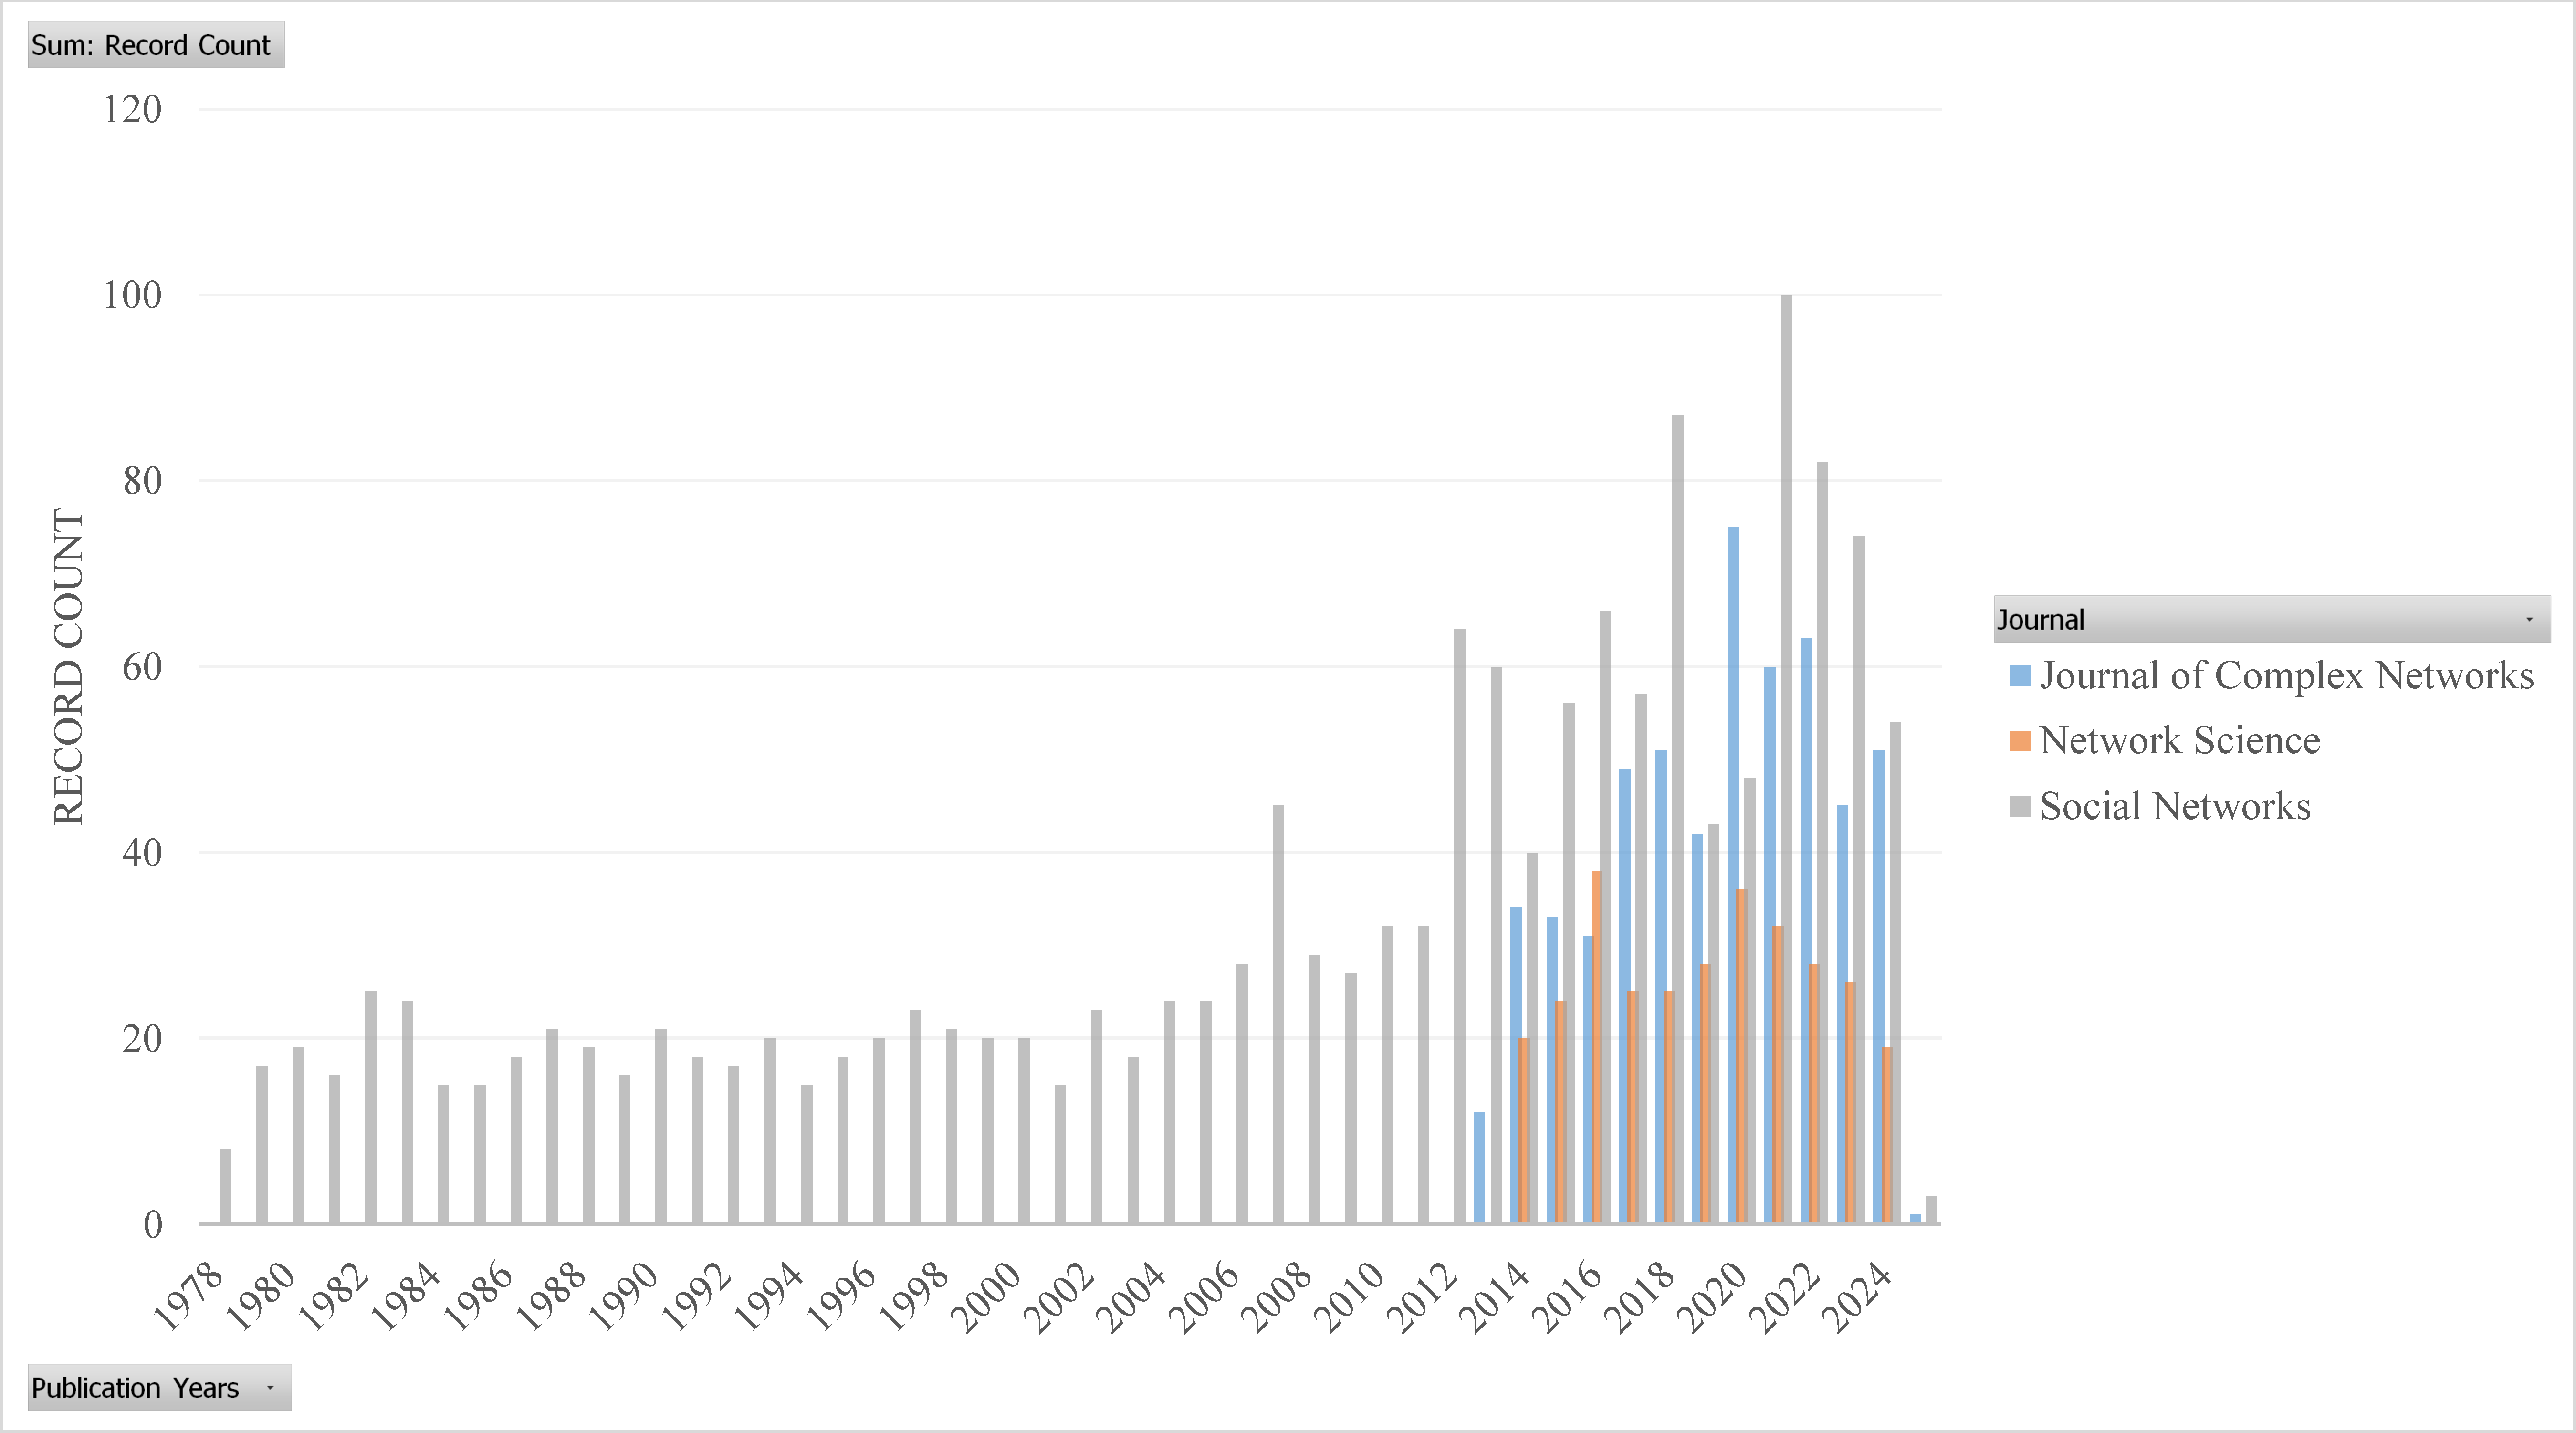
\includegraphics[width=\columnwidth]{images/Record Count Proportion.pdf}
	\end{figure}
	
	Examining the publication trajectories of \textit{Social Networks}, \textit{Journal of Complex Networks}, and \textit{Network Science} provides insight into the evolution of social network research. Figure \ref{fig.fig1} illustrates how research output has changed over time, highlighting the growth and specialization of the field.
	
	\subsubsection*{Expansion and Institutionalization of Social Network Research}
	
	\textit{Social Networks}, the longest-running journal in the field, has consistently published research since its founding in 1978. For several decades, it served as the primary outlet for social network analysis, maintaining relatively stable publication volumes. However, since 2010, a significant rise in output is observed, reflecting the increasing role of computational methods and empirical applications in network studies. This surge suggests a broadening of the field, as new methodologies and interdisciplinary collaborations have expanded the scope of research published in the journal.
	
	The introduction of \textit{Journal of Complex Networks} in 2013 signaled a growing interest in mathematical and computational models of networks. Initially publishing at a modest rate, the journal experienced rapid growth after 2015, and by 2020, its annual output was approaching that of \textit{Social Networks}. This expansion underscores the development of complex network research as a distinct subfield, drawing contributions from applied mathematics, computer science, and physics.
	
	\textit{Network Science}, launched in 2014, has a comparatively lower publication volume than the other two journals. This suggests that it may serve a more specialized academic community, focusing on foundational principles of network theory and interdisciplinary perspectives. Although its publication count has grown steadily, it remains the smallest of the three journals in terms of annual output, reinforcing its niche within the broader landscape of network science.
	
	\subsubsection*{Publication Growth and Recent Trends}
	
	Between 2016 and 2022, all three journals experienced a marked increase in publication activity, mirroring the rising academic interest in network science. During this period, \textit{Social Networks} surpassed 100 publications per year, while \textit{Journal of Complex Networks} and \textit{Network Science} followed similar trajectories on a smaller scale. This growth coincides with the expansion of big data research, computational social science, and machine learning applications, all of which have contributed to the increasing prominence of network-based methodologies.
	
	More recently, post-2022 trends indicate a decline or stabilization in publication volumes. While this could signal a saturation of research in certain areas, it is also possible that database indexing delays contribute to the observed decline. Further analysis is required to determine whether this trend reflects a plateau in network science research or a shift in thematic focus within the field.
	
	\subsubsection*{Thematic Differentiation Among Journals}
	
	The trajectories of these journals illustrate the differentiation of research themes within social network studies. \textit{Social Networks} remains the central venue for applied and empirical studies, maintaining strong connections with sociology, organizational research, and human behavior. In contrast, \textit{Journal of Complex Networks} has emerged as a leading platform for computational and mathematical approaches, while \textit{Network Science} serves as a bridge between theoretical and interdisciplinary perspectives.
	
	These patterns suggest that while network science continues to evolve as a broad field, specialization within its subdomains has led to distinct publication venues catering to different research communities. Further investigation into citation networks and thematic clustering will provide deeper insights into how these journals interact and influence one another over time.
	
	
	\subsection{Prolific Authors}\label{Prolific Authors}
	
	This section investigates the contributions of the most prolific authors within the domain of social network research, across three prominent journals: \textit{Social Networks}, \textit{Journal of Complex Networks}, and \textit{Network Science}. By analyzing the publication records, we uncover the significant roles these individuals play in shaping the field and defining its intellectual boundaries.
	
	\begin{figure*}[htbp]
		\centering
		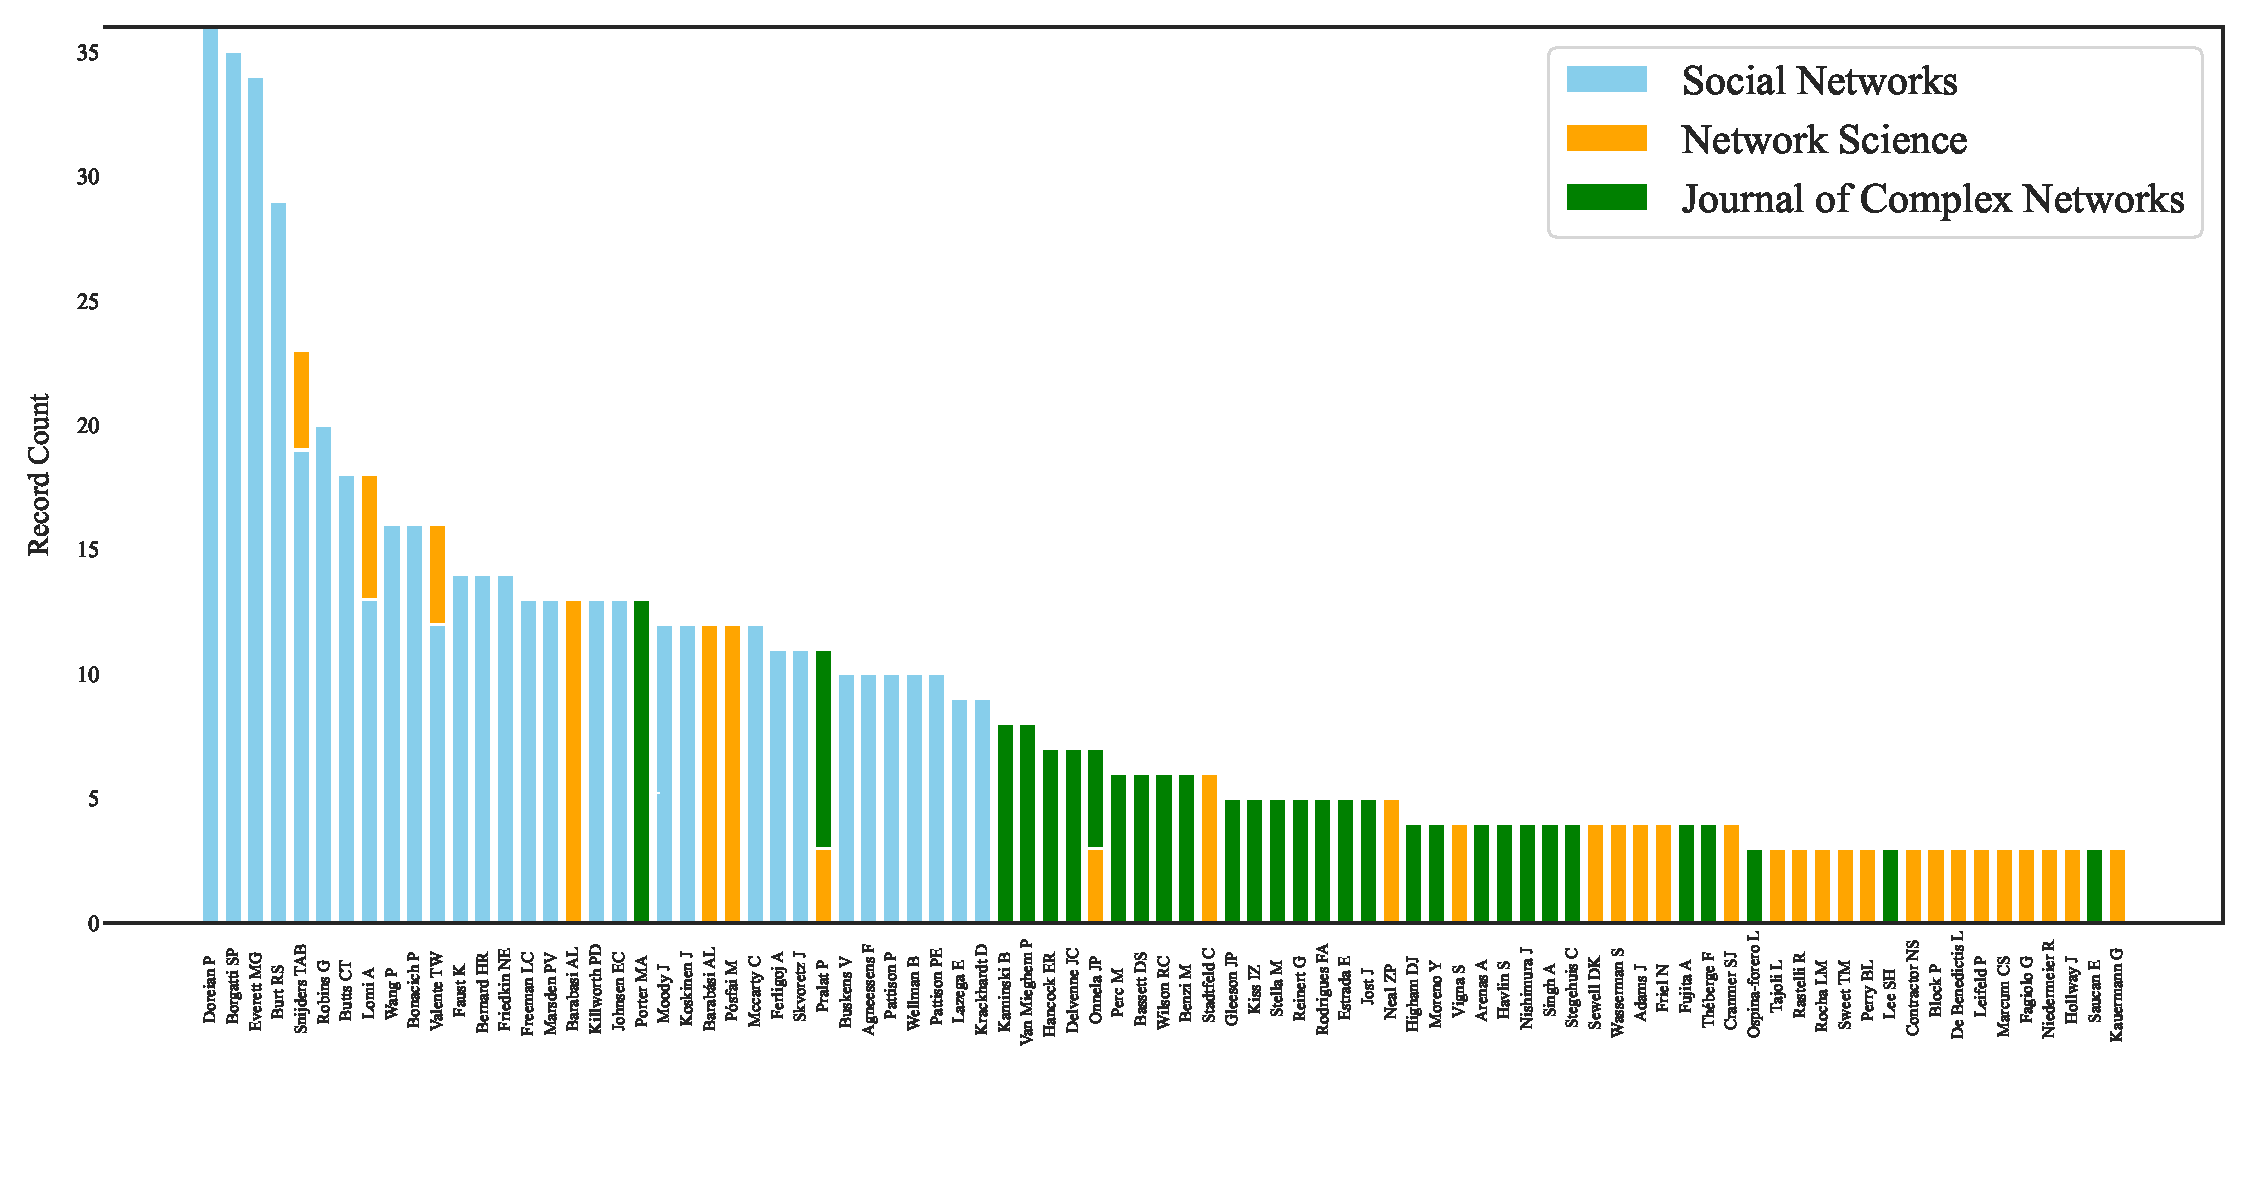
\includegraphics[width=\textwidth]{images/Top 30 Authors by Publication Count Across Three Journals.pdf}
		\caption{Prolific Authors}
		\label{fig.fig2}
	\end{figure*}
	
	\subsubsection*{Author Contributions and Research Orientations}
	
	The distribution of publications among the most prolific authors reveals distinct preferences and specializations that align closely with each journal's thematic and methodological emphases. Notably, authors like \textbf{Doreian P}, \textbf{Borgatti SP}, and \textbf{Everett MG} dominate in \textit{Social Networks}, suggesting their research aligns with traditional social network analysis, which often focuses on sociological applications and network dynamics within communities.
	
	In stark contrast, \textbf{Barabási AL} and \textbf{Porter MA} show a strong inclination towards \textit{Journal of Complex Networks} and \textit{Network Science}, indicating their work's alignment with more computational and theoretical approaches. These journals typically attract studies centered on complex systems, network theory, and often interdisciplinary approaches that draw from physics, computer science, and biology.
	
	\subsubsection*{Patterns of Specialization and Cross-Journal Engagement}
	
	The limited cross-journal publication by authors may stem from the distinct academic cultures and publication strategies inherent in their areas of expertise. It is reasonable to hypothesize that:
	\begin{itemize}
		\item \textbf{Empirical and Applied Research Focus:} Authors publishing predominantly in \textit{Social Networks} might prioritize empirical data and real-world applications, which aligns with the journal's aim to influence practical and policy-related outcomes.
		\item \textbf{Theoretical and Computational Focus:} Conversely, authors like \textbf{Porter MA} and \textbf{Barabási AL} engage with journals like \textit{Journal of Complex Networks} and \textit{Network Science} due to their interest in developing new theoretical frameworks and computational models that may not align with the more applied nature of \textit{Social Networks}.
	\end{itemize}
	
	This specialization underlines a broader academic phenomenon where researchers often become siloed within their disciplinary boundaries, occasionally leading to challenges in interdisciplinary research dissemination. The fact that very few authors publish across all three journals suggests a significant opportunity for promoting interdisciplinary research, which could bridge gaps between empirical and computational studies.
	
	\subsubsection*{Implications for the Field}
	
	This segmentation of publishing within specific journals reflects broader intellectual trends and may suggest potential barriers to interdisciplinary research. While \textit{Social Networks} continues to draw empirical research, the theoretical insights from \textit{Journal of Complex Networks} and \textit{Network Science} could enrich these empirical findings, and vice versa.
	
	The presence of a small but notable group of cross-journal contributors offers a glimpse into the potential for more integrated research approaches. By fostering interdisciplinary contributions, the field could leverage computational models to enhance empirical research, ultimately leading to more robust findings that can advance the understanding of network processes across different domains.
	
	In subsequent sections, we will delve deeper into how these publication patterns reflect the evolving landscape of network research and what they imply about the integration of methodological innovations across disciplines.
	
	\subsection{Institutional Contributions to Social Network Research}\label{Institutional Contributions to Social Network Research}
	
	This section examines the leading institutional contributors to social network research, focusing on their publication records across three key journals: \textit{Social Networks}, \textit{Journal of Complex Networks}, and \textit{Network Science}. By analyzing the top affiliations in each journal, we gain insight into dominant institutions, regional patterns, and the differing research orientations reflected in these publication venues.
	
	\subsubsection*{Institutional Influence and Regional Disparities}
	
	A clear pattern emerges in the institutional distribution of social network research. The \textit{University of California System} is the most prolific contributor, with substantial publication output across all three journals. Its presence is most pronounced in \textit{Social Networks}, where it accounts for the largest institutional share, but it also maintains a notable footprint in \textit{Journal of Complex Networks} and \textit{Network Science}. This broad engagement underscores its commitment to both empirical and computational network science.
	
	Beyond the University of California System, North American institutions dominate contributions to \textit{Social Networks}, reinforcing the journal’s strong ties to sociology and applied network analysis. Universities such as \textit{Pennsylvania Commonwealth System of Higher Education}, \textit{University of Pittsburgh}, and \textit{University of California Irvine} rank among the most frequent contributors. Meanwhile, European universities, particularly \textit{University of Groningen} and \textit{University of Oxford}, play a central role, highlighting the journal’s reach beyond the United States.
	
	\subsubsection*{Theoretical Focus in Journal of Complex Networks}
	
	In contrast, \textit{Journal of Complex Networks} features a stronger presence of European institutions, reflecting its emphasis on mathematical and algorithmic approaches to network science. The leading contributors include \textit{University of Oxford}, \textit{Centre National de la Recherche Scientifique (CNRS)}, and \textit{University of London}, institutions known for their focus on theoretical modeling and complexity science. Many of these affiliations maintain collaborations with physics and computer science departments, further reinforcing the journal’s orientation toward formal network analysis.
	
	\subsubsection*{Interdisciplinary Engagement in Network Science}
	
	\textit{Network Science} presents a more interdisciplinary institutional composition, incorporating both theoretical and applied perspectives. It attracts contributions from leading research universities, including \textit{Harvard University}, \textit{Indiana University}, and \textit{Central European University}, each of which has established itself as a center for computational and quantitative social science. Additionally, institutions such as \textit{The Santa Fe Institute} and \textit{CNRS} are well represented, reflecting the journal’s emphasis on interdisciplinary and fundamental research in network theory.
	
	\subsubsection*{Institutional Overlap and Specialization}
	
	While a few institutions maintain a presence across all three journals, most exhibit specialization in either applied or theoretical network research. Universities such as \textit{Oxford} and \textit{California} contribute broadly, spanning both empirical and computational network studies. However, others, like \textit{CNRS} and \textit{Harvard}, are more concentrated in \textit{Journal of Complex Networks} and \textit{Network Science}, respectively, signaling a stronger focus on formal network methodologies. The relative lack of institutional overlap suggests that, despite their shared focus on network research, these journals cater to distinct scholarly communities.
	
	\subsubsection*{Implications for the Field}
	
	The institutional landscape of social network research reflects both regional and disciplinary distinctions. \textit{Social Networks} remains closely linked to North American universities with strong traditions in empirical network studies, while European institutions lead contributions to \textit{Journal of Complex Networks} and \textit{Network Science}, reinforcing their prominence in complexity science and theoretical research. The presence of highly specialized institutions such as \textit{The Santa Fe Institute} highlights the growing role of interdisciplinary approaches, while increasing contributions from regions outside North America and Europe—such as \textit{Universidade de São Paulo}—signal a gradual globalization of the field.
	
	\begin{table}
		\caption{Top 10 Affiliations per Journal}
		\label{table.tab1}
		\resizebox{\linewidth}{!}{
			\begin{tabular}{lcl}
				\toprule
				Affiliations & Record Count & Journal \\
				\midrule
				UNIVERSITY OF CALIFORNIA SYSTEM               & 171 & Social Networks \\
				UNIVERSITY OF CALIFORNIA IRVINE               & 86 & Social Networks \\
				PENNSYLVANIA COMMONWEALTH SYSTEM OF HIGHER ED & 73 & Social Networks \\
				UNIVERSITY OF GRONINGEN                       & 66 & Social Networks \\
				UNIVERSITY OF OXFORD                          & 55 & Social Networks \\
				UNIVERSITY OF PITTSBURGH                      & 52 & Social Networks \\
				UTRECHT UNIVERSITY                            & 47 & Social Networks \\
				UNIVERSITY OF CHICAGO                         & 41 & Social Networks \\
				UNIVERSITY OF MELBOURNE                       & 41 & Social Networks \\
				UNIVERSITY OF SOUTH CAROLINA COLUMBIA         & 41 & Social Networks \\
				UNIVERSITY OF OXFORD                          & 30 & Journal of Complex Networks \\
				UNIVERSITY OF CALIFORNIA SYSTEM               & 21 & Journal of Complex Networks \\
				HARVARD UNIVERSITY                            & 20 & Network Science \\
				UNIVERSITY OF CALIFORNIA SYSTEM               & 18 & Network Science \\
				CENTRE NATIONAL DE LA RECHERCHE SCIENTIFIQUE  & 18 & Journal of Complex Networks \\
				UNIVERSITY OF LONDON                          & 16 & Journal of Complex Networks \\
				INDIANA UNIVERSITY BLOOMINGTON                & 15 & Network Science \\
				INDIANA UNIVERSITY SYSTEM                     & 15 & Network Science \\
				NORTHEASTERN UNIVERSITY                       & 15 & Network Science \\
				CENTRAL EUROPEAN UNIVERSITY                   & 14 & Network Science \\
				UNIVERSIDADE DE SAO PAULO                     & 14 & Journal of Complex Networks \\
				CENTRE NATIONAL DE LA RECHERCHE SCIENTIFIQUE  & 13 & Network Science \\
				THE SANTA FE INSTITUTE                        & 13 & Journal of Complex Networks \\
				HARVARD MEDICAL SCHOOL                        & 12 & Network Science \\
				UNIVERSITY OF OXFORD                          & 12 & Network Science \\
				MAX PLANCK SOCIETY                            & 11 & Journal of Complex Networks \\
				UNIVERSITY OF CALIFORNIA LOS ANGELES          & 11 & Journal of Complex Networks \\
				UNIVERSITY OF TRENTO                          & 11 & Journal of Complex Networks \\
				UNIVERSITY OF GRONINGEN                       & 10 & Network Science \\
				MASSACHUSETTS INSTITUTE OF TECHNOLOGY MIT     & 10 & Journal of Complex Networks \\
				\bottomrule
		\end{tabular}}
	\end{table}

	
	
	\subsection{Country/Region-Level Contributions}
	
	The geographic distribution of research output provides insights into the global development and dissemination of social network research. By analyzing the contributions of countries to the three selected journals—Social Networks, Journal of Complex Networks, and Network Science—we can identify regional hubs of academic activity and collaboration. This subsection examines the country-level publication data to highlight the dominant contributors to the field, emerging regions of influence, and the role of international collaboration in advancing social network research. Understanding these patterns is crucial for contextualizing the field's intellectual and geographic diversity.
	
	We'll start with the result in Table then the interpretation.
	
	\bibliographystyle{apalike}
	\bibliography{ref}
	
\end{document}
